\chapter{Summary and Outlook}
\markboth{Summary and Outlook}{Summary and Outlook}

This book takes `symmetry $\to$ invariant $\to$ closed orbit $\to$ period' as its guiding principle, and constructs a mathematical framework that unifies periodic phenomena starting from first principles. The core methodology of the book rests on four pillars: \textbf{group representation theory} supplies the algebraic foundation of periodic structure, \textbf{periodic convolution} supplies a unified computational framework for phase interaction across periods, \textbf{the window-function and refractive-index system} supplies turning-point diagnostic tools based on similarity and tendency, and \textbf{the complex exponential activation function (CEAF) together with kernel-smoothed derivative-integral descent} supplies learnable nonlinearities with intrinsic periodic structure and multiscale optimisation algorithms.

The journey of the book begins with the mathematical characterisation of three fundamental centres of symmetry---$0$, $1$ and $i$---passes through group representation theory, vector analysis, harmonic analysis, periodic manifolds and periodic categories, proceeds by way of the construction of periodic convolution and of the window-function--refractive-index system, and ends with systematic applications in such domains as astronomy, calendars, geography, physics, biology, psychology, economics, politics, cryptography, agents and data analysis, thereby forming a self-consistent theoretical system that runs from discrete information processing to continuous physical laws and from physical dynamics to life and society.

\begin{remark}[Positioning of this chapter]\label{rem:summary_chapter_positioning}
This chapter is the closing chapter of the book. The preceding 45 chapters have respectively established: one main chain (symmetry $\to$ invariant $\to$ closed orbit $\to$ period), three groups of support (group representation theory, periodic convolution, the window-function and refractive-index system, and complex exponential activation with kernel-smoothed derivative-integral descent), and instantiations in more than twenty domains. The task of this chapter is not to introduce new tools but to undertake a \textbf{horizontal comparison}: to place the main chain, the four pillars and the seven themes of the various chapters of the book side by side in one set of tables, and to point out which conclusions have already been proved rigorously, which still belong to a research programme, and which are unsolved problems. The reader may read this chapter first in order to obtain a global map, and then return to the individual chapters.

Positioning of the seven themes in this chapter: \textbf{translation}---the book takes the translation group as the most fundamental evolution group; \textbf{scaling}---scaling and logarithmic coordinates run through the number systems, harmonic analysis and time series; \textbf{rotation}---phase and roots of unity are the core carriers of periodic structure; \textbf{conservation}---the correspondence between symmetry and conservation is the logical hub of the book; \textbf{symmetry}---the unity of the group-action framework; \textbf{closure}---closed orbits are the geometric criterion of periodicity; \textbf{period}---the theme of the book itself.
\end{remark}

\section{Looking back: one main chain and three groups of support}

If the theoretical through-line of the whole book were to be summarised in a single sentence, it would be this:

\begin{center}
\textbf{Finite-order action gives periodicity; conservation and symmetry help to discover, constrain and explain periodicity; periodic convolution, window functions--refractive index, and CEAF--KDI supply computational, diagnostic and learning tools respectively.}
\end{center}

This main line is established rigorously in the `Operations and Periodicity' chapter: iteration is the starting point, invariants and conservation characterise the stratification between orbits, symmetry is a transformation that commutes with the evolution, finite-order action directly produces uniformly closed orbits, and a closed orbit is equivalent to pointwise periodicity. A conserved quantity is not a necessary condition for periodicity, nor is it in general a sufficient one; in conservative systems it is associated with continuous symmetries through Noether's theorem and supplies constraints on and explanations of periodic structure, but the algebraic hub that directly produces periodicity is finite-order action.

\begin{figure}[htbp]
\centering
\begin{tikzpicture}[
  node distance=1.5cm and 2.0cm,
  every node/.style={font=\small},
  >=stealth,
  main/.style={draw, rounded corners=3pt, fill=blue!8, minimum width=2.2cm, minimum height=0.85cm, align=center},
  aux/.style={draw, rounded corners=3pt, fill=green!8, minimum width=2.6cm, minimum height=0.75cm, align=center, font=\footnotesize, text width=2.4cm},
  arrow/.style={-{stealth}, thick},
  auxarrow/.style={-{stealth}, thick, dashed, green!50!black}
]
\node[main] (iter) {Iteration};
\node[main, right=of iter] (inv) {Invariants/conservation};
\node[main, right=of inv] (sym) {Symmetry};

\node[main, below=of sym] (fin) {Finite-order action};
\node[main, left=of fin] (clo) {Closed orbit};
\node[main, left=of clo] (per) {Period};

\draw[arrow] (iter) -- (inv);
\draw[arrow] (inv) -- (sym);
\draw[arrow] (sym) -- (fin);
\draw[arrow] (fin) -- (clo);
\draw[arrow] (clo) -- (per);

\node[aux, above=of inv] (cons) {Conserved quantities: constraining orbits, stratification};
\node[aux, above=of sym] (symaux) {Symmetry group: centraliser, group action};
\draw[auxarrow] (cons) -- (inv);
\draw[auxarrow] (symaux) -- (sym);

\node[font=\footnotesize, align=center] at (2.0,-4.2) {Conservation and symmetry are auxiliary tools, not unavoidable links in the chain of periodicity};
\end{tikzpicture}
\caption{The main logical chain of the book: iteration $\to$ invariants/conservation $\to$ symmetry $\to$ finite-order action $\to$ closed orbit $\to$ period. Conservation and symmetry are attached by dashed lines, indicating their auxiliary status.}
\label{fig:closing_main_chain}
\end{figure}

This main chain unfolds downwards into three levels: the \textbf{algebraic level} studies finite-order action, group representations and the automorphism tower; the \textbf{geometric level} studies manifolds, fibre bundles, periodic manifolds and closed orbits; and the \textbf{analytic level} studies series, convolution, harmonic analysis, sampling and intercalation. Together the three support the interdisciplinary diagnosis of the application level.

\section{The architecture of the book's theoretical system}

\begin{figure}[htbp]
    \centering
    \adjustbox{max width=\textwidth}{%
    \begin{tikzpicture}[>=stealth,
        layer/.style={draw, rounded corners, minimum width=2.8cm, minimum height=0.9cm, align=center, font=\small},
        core/.style={draw, rounded corners, fill=blue!10, minimum width=2.8cm, minimum height=0.9cm, align=center, font=\small\bfseries},
        tool/.style={draw, rounded corners, fill=green!10, minimum width=2.8cm, minimum height=0.9cm, align=center, font=\small},
        app/.style={draw, rounded corners, fill=red!10, minimum width=2.2cm, minimum height=0.8cm, align=center, font=\scriptsize},
        arrow/.style={->, thick, >=stealth}]
        
        \node[core] (c0) at (-3, 0) {Centre of symmetry $0$\\additive symmetry};
        \node[core] (c1) at (0, 0) {Centre of symmetry $1$\\multiplicative symmetry};
        \node[core] (ci) at (3, 0) {Centre of symmetry $i$\\rotational symmetry};
        
        \node[layer, fill=blue!5] (num) at (-7.5, -2) {Number systems\\$\mathbb{N}\to\mathbb{Z}\to\mathbb{Q}$\\$\to\mathbb{R}\to\mathbb{C}\to\mathbb{H}$};
        \node[layer, fill=blue!5] (grp) at (-3.75, -2) {Groups and group functions\\8 pairs of concepts\\transitivity matrix};
        \node[layer, fill=blue!5] (vec) at (0, -2) {Scalars and vectors\\12 similarities\\12 tendencies};
        \node[layer, fill=blue!5] (ana) at (3.75, -2) {Functions and analysis\\limit angle\\differential similarity\\integral tendency};
        \node[layer, fill=blue!5] (lin) at (7.5, -2) {Linear algebra\\spectral theorem\\matrix groups\\SVD};
        
        \node[layer, fill=green!5] (prob) at (-7.5, -4.5) {Probability theory\\phase mass assignment\\Bayesian updating};
        \node[layer, fill=green!5] (vf) at (-3.75, -4.5) {Vector analysis\\flux model\\epicycles\\derivative-integral descent};
        \node[layer, fill=green!5] (pfunc) at (0, -4.5) {Periodic functions and groups with periodic orbits\\nested epicycles\\phase operators};
        \node[layer, fill=green!5] (harm) at (3.75, -4.5) {Harmonic analysis\\periodic convolution\\periodic tendency spectrum};
        \node[layer, fill=green!5] (manifold) at (7.5, -4.5) {Periodic manifolds\\discrete lattice points\\discrete unitary};
        
        \node[core] (system) at (-3, -7) {Periodic systems\\composite periods\\invariants};
        \node[core] (category) at (0, -7) {Periodic categories\\functors and natural transformations};
        \node[core] (method) at (4, -7) {Modelling and analysis\\CEAF + derivative-integral descent};
        
        \node[app] (a1) at (-9, -9.5) {Astronomy};
        \node[app] (a2) at (-6.5, -9.5) {Calendars};
        \node[app] (a3) at (-4, -9.5) {Geography};
        \node[app] (a4) at (-1.5, -9.5) {The I Ching};
        \node[app] (a5) at (1, -9.5) {Electromagnetism};
        \node[app] (a6) at (3.5, -9.5) {Audio};
        \node[app] (a7) at (6, -9.5) {Mechanics};
        \node[app] (a8) at (8.5, -9.5) {Circuits and chips};
        
        \node[app] (b1) at (-9, -11) {Biology};
        \node[app] (b2) at (-6.5, -11) {Psychology};
        \node[app] (b3) at (-4, -11) {Social interaction};
        \node[app] (b4) at (-1.5, -11) {Climate};
        \node[app] (b5) at (1, -11) {Economics};
        \node[app] (b6) at (3.5, -11) {Politics};
        \node[app] (b7) at (6, -11) {Data analysis};
        \node[app] (b8) at (8.5, -11) {Agent algorithms};
        
        \draw[arrow] (c0) -- (grp);
        \draw[arrow] (c0) -- (num);
        \draw[arrow] (c1) -- (vec);
        \draw[arrow] (c1) -- (ana);
        \draw[arrow] (ci) -- (lin);
        
        \draw[arrow] (num) -- (prob);
        \draw[arrow] (grp) -- (vf);
        \draw[arrow] (vec) -- (pfunc);
        \draw[arrow] (ana) -- (harm);
        \draw[arrow] (lin) -- (manifold);
        
        \draw[arrow] (prob) -- (system);
        \draw[arrow] (vf) -- (system);
        \draw[arrow] (pfunc) -- (category);
        \draw[arrow] (harm) -- (category);
        \draw[arrow] (manifold) -- (method);
        
        \draw[arrow] (system.south) -- (a4.north);
        \draw[arrow] (system.south) -- (b4.north);
        \draw[arrow] (category.south) -- (a5.north);
        \draw[arrow] (category.south) -- (b5.north);
        \draw[arrow] (method.south) -- (a7.north);
        \draw[arrow] (method.south) -- (b7.north);
        
        \node[font=\small\bfseries, blue!60!black, left=0.1cm of c0, xshift=-0.8cm] {Centres of symmetry};
        \node[font=\small\bfseries, blue!60!black, left=0.1cm of num, xshift=-1.2cm] {Mathematical foundations};
        \node[font=\small\bfseries, green!60!black, left=0.1cm of prob, xshift=-1.2cm] {Core theory};
        \node[font=\small\bfseries, purple!60!black, left=0.1cm of system, xshift=-1.2cm] {Unified framework};
        \node[font=\small\bfseries, red!60!black, left=0.1cm of a1, xshift=-1.2cm] {Application domains};
    \end{tikzpicture}%
    }
    \caption{Architecture diagram of the theoretical system of the whole book on periodic mathematics. Starting from the centres of symmetry, passing through the mathematical foundations and the core theory, unified in periodic systems, periodic categories and the methodology of modelling and analysis, and finally applied in the various disciplines.}
    \label{fig:architecture_summary}
\end{figure}

From the point of view of chapter structure, the book may be divided into three parts, with the present chapter serving as its close:

\begin{center}
\renewcommand{\arraystretch}{1.25}
\begin{tabular}{@{}p{3.2cm}p{8.5cm}@{}}
\toprule
\textbf{Part} & \textbf{Main content} \\
\midrule
Mathematical foundations and generators & Foundations of periodicity, number systems, scalars and vectors, functions and limits, differential equations and complex functions, series and convolution \\
Core structures, tools and methods & Linear algebra, foundations of manifolds and fibre bundles, periodic manifolds, periodic categories, probability theory, vector analysis, groups and group functions, higher-order groups and higher-order functions, periodic functions and groups with periodic orbits, discrete sampling approximation and intercalation, harmonic analysis, time series analysis, periodic systems \\
Interdisciplinary applications and diagnosis & Probability, cryptography, astronomy, calendars, geography, the I Ching, electromagnetism, audio, mechanics, circuits and chips, biology, psychology, social interaction, climate, economics, politics, data analysis, agents, algorithms, modelling and analysis \\
\bottomrule
\end{tabular}
\end{center}

Among these, the `Periodic Systems' chapter is the bridging chapter that leads from pure mathematics to applied mathematics. It provides the five-step interface by which an arbitrary target is connected to the framework of periodic mathematics: \textbf{decision} (whether the target is periodic, and its period type), \textbf{construction} (building the amplitude series, the frequency series and the phase series from the turning points, and assembling the epicycle group), \textbf{adjustment} (dynamically adjusting the number and the parameters of the epicycles), \textbf{convolution} (amplitude convolution, phase convolution and frequency convolution), and \textbf{integration} (connecting to the tool chains of sampling, harmonic analysis and time series analysis). Every subsequent application chapter develops along this interface.

\section{Relations among the four pillars}

\begin{figure}[htbp]
    \centering
    \adjustbox{max width=\textwidth}{%
    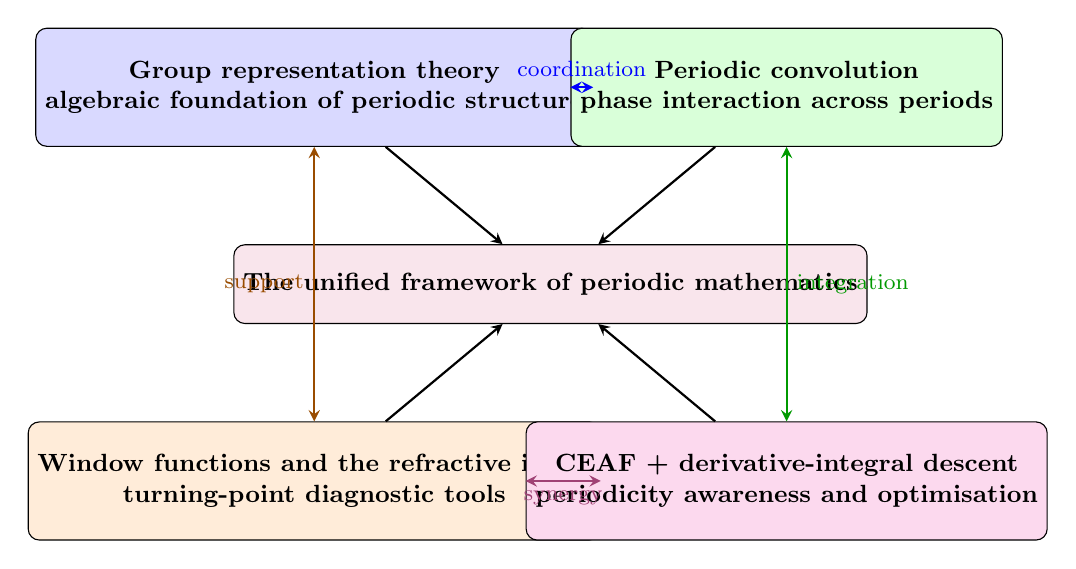
\begin{tikzpicture}[>=stealth,
        pillar/.style={draw, rounded corners, fill=blue!10, minimum width=3.5cm, minimum height=1.5cm, align=center, font=\small\bfseries},
        arrow/.style={->, thick, >=stealth}]
        
        \node[pillar, fill=blue!15] (group) at (0, 2.5) {Group representation theory\\algebraic foundation of periodic structure};
        \node[pillar, fill=green!15] (full) at (6, 2.5) {Periodic convolution\\phase interaction across periods};
        \node[pillar, fill=orange!15] (window) at (0, -2.5) {Window functions and the refractive index\\turning-point diagnostic tools};
        \node[pillar, fill=magenta!15] (eaf) at (6, -2.5) {CEAF + derivative-integral descent\\periodicity awareness and optimisation};
        
        \node[draw, rounded corners, fill=purple!10, minimum width=5cm, minimum height=1cm, align=center, font=\small\bfseries] (core) at (3, 0) {The unified framework of periodic mathematics};
        
        \draw[arrow] (group) -- (core);
        \draw[arrow] (full) -- (core);
        \draw[arrow] (window) -- (core);
        \draw[arrow] (eaf) -- (core);
        
        \draw[<->, thick, blue] (group.east) -- (full.west) node[midway, above, font=\footnotesize] {coordination};
        \draw[<->, thick, green!60!black] (full.south) -- (eaf.north) node[midway, right, font=\footnotesize] {integration};
        \draw[<->, thick, orange!60!black] (window.north) -- (group.south) node[midway, left, font=\footnotesize] {support};
        \draw[<->, thick, magenta!60!black] (window.east) -- (eaf.west) node[midway, below, font=\footnotesize] {synergy};
    \end{tikzpicture}%
    }
    \caption{Relations among the four pillars of periodic mathematics.}
    \label{fig:four_pillars}
\end{figure}

The four pillars are not independent of one another. Group representation theory answers `what is the algebraic form of periodic structure'; periodic convolution answers `how do different periods interact with one another'; window functions and the refractive index answer `how are turning points, reversals and leakage diagnosed from data'; and CEAF and KDI answer `how is periodic structure turned into a learnable, optimisable computational unit'. The four are linked together through the common objects `phase operator', `epicycle group', `periodic series' and `Waveform'.

\section{Periodic convolution: a unified framework for phase interaction across periods}

\textbf{Periodic convolution} is one of the important methodological frameworks of this book. The five-stage ladder of the book---\textbf{convolution} (two functions and a delay are passed in, and delay products are computed), \textbf{similarity convolution} (cosine similarity and sine similarity are packed into a complex matrix), \textbf{trend convolution} (the similarity convolutions multiplied by each other's moduli), \textbf{the periodic series} (a complex series whose components are the four-tuple of amplitude, frequency, phase and period), \textbf{periodic convolution} (all four parameters acting as operators)---unifies the traditional integral transforms (the Fourier series, the Fourier transform, the DFT, the FFT, the wavelet transform, the Mellin transform, the Laplace transform, the chirp-Z transform and the Hilbert transform) as special cases of the periodic transform and of periodic convolution under a specific dictionary, kernel and algorithmic realisation, and completes the information on phase interaction that the traditional methods discard.

\begin{figure}[htbp]
\centering
\begin{tikzpicture}[
  node distance=0.8cm,
  every node/.style={font=\small},
  >=stealth,
  ladder/.style={draw, rounded corners=3pt, minimum width=8.5cm, minimum height=0.8cm, align=center},
  arrow/.style={-{stealth}, thick}
]
\node[ladder, fill=blue!8] (s1) {Classical convolution: retains only the delay products of equal-frequency pairs $m=n$};
\node[ladder, fill=cyan!10, below=of s1] (s2) {Phase convolution / amplitude convolution / frequency convolution: retains the phase, amplitude and frequency components of all frequency pairs};
\node[ladder, fill=green!10, below=of s2] (s3) {Trend convolution: retains the amplitudes and phases of all frequency pairs};
\node[ladder, fill=orange!10, below=of s3] (s4) {Periodic series: decomposition into multiple period layers, the four-tuple $(A_{p,n},\omega_{p,n},\phi_{p,n},T_p)$};
\node[ladder, fill=red!10, below=of s4] (s5) {Periodic convolution: the four-parameter operator, retaining the interaction of all frequency pairs and all period pairs};

\draw[arrow] (s1) -- (s2);
\draw[arrow] (s2) -- (s3);
\draw[arrow] (s3) -- (s4);
\draw[arrow] (s4) -- (s5);

\node[font=\footnotesize, align=center] at (0,-6.0) {The five-stage ladder: information increases level by level, and each level is a degeneration or a generalisation of the level above};
\end{tikzpicture}
\caption{The five-stage ladder of periodic convolution.}
\label{fig:closing_convolution_ladder}
\end{figure}

The core formula of periodic convolution is:
\[
(f \circledast g)(\tau) = \sum_{p,q} \Theta_{p,q} \sum_{n,m} W(\omega_{p,n} - \nu_{q,m}) \cdot (A_{p,n} B_{q,m})^{\alpha} \cdot S^{(d)}(\phi_{p,n}, \psi_{q,m}) \cdot e^{i\nu_{q,m} \tau},
\]
in which the four factors are respectively the \textbf{amplitude operator} (scaling, with the switch $\alpha$), the \textbf{phase operator} (rotation, with 6 complex phase kernels $S^{(d)}$), the \textbf{frequency operator} (translation, with the weight kernel $W$ and the delay phase factor $e^{i\nu\tau}$), and the \textbf{period operator} (fixed length, with the period-pair weight $\Theta_{p,q}$).

The degeneration chain of periodic convolution---classical convolution/cross-correlation (the kernel-width limit $W \to \delta$), similarity convolution ($\alpha = 0$), trend convolution ($\alpha = 1$) and kernelised convolution (the single-period layer)---constitutes a complete analytical tool chain from the time domain to the frequency domain and from a single period to multi-period coupling. The classical limit of the periodic tendency spectrum is the power spectrum, and the Fisher test gives an exact threshold for period significance.

The introduction of the concept of a \textbf{phase operator} reveals that every phase of every period is a kind of relational operator: $\mathcal{O}_k^{(T)} = e^{i2\pi k/T}$ not only marks a position, but defines a relation through complex multiplication. Multiplication by $\mathcal{O}_0 = 1$ (the yang operator) gives the object itself (congruence), multiplication by $\mathcal{O}_{T/2} = -1$ (the yin operator) gives the opposite vector (hedging), and multiplication by an arbitrary $\mathcal{O}_k$ defines the relation of rotation by $2\pi k/T$.

\textbf{The epicycle nesting generation rule}---for every single step forward of the outer circle, the inner circle rotates through one full turn---unifies the process by which a small period generates a large period: Yin-Yang $\times$ the Five Phases = the Heavenly Stems ($10$), the Four Symbols $\times$ Sancai = the Earthly Branches ($12$), and the Eight Trigrams $\times$ the Eight Trigrams = the Sixty-Four Hexagrams ($64$). The sexagenary cycle is generated by the periodic convolution of the Heavenly Stems and the Earthly Branches.

\section{Window functions and the refractive index: turning-point diagnosis based on similarity and tendency}

\textbf{The window-function and refractive-index system} is another important methodological framework of this book. It generalises the geometric prototypes of the law of reflection and the law of refraction to the trend analysis of time series, and thereby establishes a tool chain for turning-point diagnosis based on similarity and tendency.

\begin{figure}[htbp]
\centering
\begin{tikzpicture}[
  node distance=0.8cm and 0.8cm,
  every node/.style={font=\small},
  >=stealth,
  box/.style={draw, rounded corners=3pt, fill=blue!8, minimum width=2.4cm, minimum height=0.8cm, align=center},
  arrow/.style={-{stealth}, thick}
]
\node[box] (data) {Raw time series};
\node[box, right=of data] (smooth) {Window-function smoothing\\$T_\Delta(t)$};
\node[box, right=of smooth] (angle) {Instantaneous limit angle\\$\theta_t=\arctan(\nabla \tilde X_t)$};

\node[box, below=of angle] (sim) {Similarity\\$\cos(\Delta\theta),\sin(\Delta\theta)$};
\node[box, left=of sim] (turn) {Refraction rate\\$R_{\mathrm{turn}}$};
\node[box, left=of turn] (refr) {Refractive index\\$\eta=\sin\theta_1/\sin\theta_2$};

\draw[arrow] (data) -- (smooth);
\draw[arrow] (smooth) -- (angle);
\draw[arrow] (angle) -- (sim);  
\draw[arrow] (sim) -- (turn);  
\draw[arrow] (turn) -- (refr); 
\end{tikzpicture}
\caption{The window-function--refractive-index turning-point diagnostic procedure.}
\label{fig:closing_window_refraction}
\end{figure}

The window function $K_\Delta$ smooths a time series at multiple scales and extracts the trend component $T_\Delta(t)$. The direction sequence is then obtained through the instantaneous limit angle $\theta_t = \arctan(\nabla \tilde{X}_t)$. The turning-point criterion is: $|\theta_t - \theta_{t-1}| > \tau$ if and only if the basic difference-angle cosine similarity $\cos(\theta_t - \theta_{t-1}) < \cos\tau$; the sign of the double-angle direction similarity $\sin 2(\theta_t - \theta_{t-1})$ gives the sense of the turn, and its absolute value gives the strength of the turning point. The refraction rate $R_{\text{turn}} = |\sin\theta_1 - \sin\theta_2|$ measures the difference of the sine tendencies on the two sides of the turning point, and its half-angle decomposition is
\[
R_{\text{turn}} = 2\left|\cos\frac{\theta_1+\theta_2}{2}\right| \cdot \left|\sin\frac{\theta_1-\theta_2}{2}\right|.
\]
The refractive-index ratio $\eta = \sin\theta_1/\sin\theta_2$ serves as a formal analogue of Snell's law $n_1\sin\theta_1 = n_2\sin\theta_2$---no physical refractive index exists in a time series, and $\eta$ is used only in the sense of an analogy; the direction reversal $\theta_2 = -\theta_1$ corresponds to the `total internal reflection' analogy, in which case $R_{\text{turn}} = 2|\sin\theta_1|$. The concept of delay relates phase to time shift: the phase delay $\tau = \phi/\omega$ converts a rotational phase into a time shift, and the propagation delay $\tau = r/c$ converts a spatial distance into a time shift.

\section{The complex exponential activation function and kernel-smoothed derivative-integral descent}

\textbf{The complex exponential activation function (CEAF)} turns the nested epicycle system into a learnable activation function for neural networks:
\[
\mathcal{E}(x) = \sum_{k=1}^{N} A_k e^{i(\omega_k x + \phi_k)}.
\]
The complex-valued output of the CEAF preserves phase information naturally, and its derivative does not vanish identically on the whole real axis. Its parameters $\{A_k,\omega_k,\phi_k\}$ can be initialised from estimates obtained at the data-analysis stage---periodogram peaks, phase-coupling networks and derivative-integral descent---and then updated by backpropagation or by KDI. In this way, periodic structure extracted from data can enter a neural network end to end.

\begin{figure}[htbp]
\centering
\begin{tikzpicture}[
  node distance=1.2cm and 1.2cm,
  every node/.style={font=\small},
  >=stealth,
  box/.style={draw, rounded corners=3pt, fill=blue!8, minimum width=2.6cm, minimum height=0.85cm, align=center},
  arrow/.style={-{stealth}, thick},
  back/.style={-{stealth}, thick, dashed, blue}
]
\node[box] (data) {Data\\time series};
\node[box, right=of data] (spec) {Spectral initialisation\\$\omega_k^{(0)}$};

\node[box, below=of spec] (ceaf) {CEAF network\\$\mathcal E(x)$};
\node[box, left=of ceaf] (kdi) {KDI optimisation\\$A_k,\omega_k,\phi_k$};
\node[box, left=of kdi] (wave) {Waveform\\complex function};
\node[box, left=of wave] (pred) {Prediction and diagnosis};

\draw[arrow] (data) -- (spec);
\draw[arrow] (spec) -- (ceaf); 
\draw[arrow] (ceaf) -- (kdi);  
\draw[arrow] (kdi) -- (wave); 
\draw[arrow] (wave) -- (pred); 

\draw[back] (pred.west) to[bend left=70] 
    node[midway, above, font=\footnotesize] {feedback: residual diagnosis and parameter re-estimation} 
    (data.west);
\end{tikzpicture}
\caption{The CEAF--KDI learning loop: from data to Waveform, and back to data diagnosis.}
\label{fig:closing_ceaf_kdi_loop}
\end{figure}

\textbf{The kernel-smoothed derivative-integral descent method} exploits $N$-th order derivative and $N$-th order integral information simultaneously through a kernel function. The curvature correction term uses the second derivative to detect changes in curvature, and the cumulative-change correction term uses integral information to detect long-term trends. For the CEAF parameters, the amplitude $A_k$ is suited to smooth adjustment by a Gaussian kernel, the frequency $\omega_k$ is suited to curvature sensing by a Mexican-hat kernel, and the phase $\phi_k$ is suited to jump detection by a Hilbert kernel.

\textbf{The crystal oscillator as a fundamentally fixed epicycle} is the core observation concerning the periodic structure of chip systems: the crystal oscillator outputs an epicycle whose amplitude, frequency and phase are all fixed, and it is the master epicycle of all the other epicycles within the chip. A phase-locked loop realises frequency scaling of an epicycle, a clock tree is a nested epicycle system, and a chip is a parametrised epicycle waveform/spectrum processing unit.

\section{The logical closed loop of the book}

\begin{remark}[The logical closed loop of the book (empirical observation / research programme)]\label{thm:closing_loop}
Periodic mathematics starts from the three centres of symmetry $0$, $1$ and $i$, passes through the extension of the number systems, group representation theory, vector analysis and the flux model, periodic convolution, periodic systems, periodic manifolds and periodic categories, and finally arrives at the various application systems, thereby proposing the following \textbf{research programme} for a theoretical closed loop:
\begin{enumerate}[label=(\roman*)]
    \item Starting from the rotational symmetry $i$, the complete Maxwell equations and charge conservation are derived through local $U(1)$ gauge invariance---the electromagnetic system is the purest realisation of the rotation operation in physics (proved; see Theorem \ref{thm:maxwell_equations} in the chapter `Periodic Structure of Electromagnetic Systems').
    \item Starting from the translational symmetry $0$, energy conservation is derived through time-translation invariance---the translation operation drives the generation and maintenance of periodic structure in mechanical systems, circuit systems and climate systems (proved; see Theorem \ref{thm:mechanical_conservation} in the chapter `Periodic Structure of Mechanical Systems').
    \item Starting from the scaling symmetry $1$, scale invariance yields the \textbf{existence of a power-law exponent}---scale invariance gives the existence of the exponent, whilst its stability across periods remains an \textbf{empirical fact} (an \textbf{empirical observation / research programme}; see \ref{prop:pareto_growth} in the chapter `Periodic Structure of Economic Systems' and \ref{thm:biological_conservation} in the chapter `Periodic Structures in Biological Systems'; the stability claim in the former is itself annotated there as an empirical observation and analogical explanation, not a mathematical theorem).
\end{enumerate}
This `closed loop' is therefore an overall description of the structure of the book and a \textbf{research programme}, not a proved theorem: threads (i) and (ii) each correspond to a theorem of the respective chapter, whilst the link `stability of the scaling exponent across periods' in (iii) is an empirical observation / research programme. The three threads correspond respectively to standard results in Lagrangian mechanics, Noether's theorem and power-law scaling analysis, whose rigorous statements are given in the theorems of the corresponding chapters.
\end{remark}

\section{A unified diagnostic matrix for interdisciplinary applications}

The application chapters of the book are not isolated from one another; rather, they share one and the same diagnostic matrix. The table below lists the main application domains together with their dominant centre of symmetry, their typical period type and their main tools, so that the reader may grasp the overall layout of the book's applications.

\begin{center}
\renewcommand{\arraystretch}{1.25}
\small
\begin{tabular}{@{}p{2.2cm}p{2.5cm}p{3.2cm}p{4.8cm}@{}}
\toprule
\textbf{Domain} & \textbf{Dominant centre of symmetry} & \textbf{Typical period type} & \textbf{Main tools} \\
\midrule
Astronomy & $i$, $0$ & Orbital periods, resonance, many-body quasi-periodicity & Kepler's laws, Floquet, KAM, periodic convolution \\
Calendars & $0$, $1$ & Tropical year, synodic month, the sexagenary cycle & Intercalation, continued fractions, congruence angles, periodic convolution \\
Geography & $i$, $1$ & Milankovitch cycles, ENSO, seasonal cycles & Multiscale windows, spectral analysis, cross-scale resonance \\
The I Ching & $i$, $0$, $1$ & Hexagram periods, sexagenary periods, He Tu and Lo Shu & Phase operators, epicycle nesting, periodic convolution \\
Electromagnetism & $i$ & Electromagnetic waves, oscillation, retarded potentials & Maxwell's equations, vector analysis, delay \\
Audio & $0$, $i$ & Simple harmonic motion, harmonics, beats & Fourier series, equal temperament, delay \\
Mechanics & $0$, $i$ & Spring oscillators, the simple pendulum, resonance, precession & Limit cycles, elliptic integrals, phase response \\
Circuits and chips & $i$, $0$ & Crystal oscillators, PLLs, clock trees, data periods & Epicycles, phase-locked loops, nested clocks \\
Biology & $i$, $1$ & Circadian rhythms, heart rate, the cell cycle, population cycles & Limit cycles, delayed feedback, Lotka--Volterra \\
Psychology & $0$, $i$ & Sleep cycles, attentional oscillations, mood cycles & Two-process model, RC charge--discharge, phase locking \\
Social interaction & $i$ & Social rhythms, information propagation, collective synchronisation & SIR/SIRS, Kuramoto, phase-coupling networks \\
Climate & $i$, $1$ & Seasons, ENSO, PDO, IOD, Milankovitch & Red noise, the Hurst exponent, multitaper spectral estimation \\
Economics & $1$, $i$ & Inventory cycles, investment cycles, long waves & Multiplier--accelerator, the cobweb model, window-function diagnosis \\
Politics & $0$, $i$ & Dynastic cycles, hegemony cycles, unification--division & Positive feedback, fiscal decay, nested periods \\
Data analysis & $i$, $1$ & Periodogram peaks, multi-window decomposition, phase coupling & Periodic convolution, multitaper spectra, phase networks \\
Agent algorithms & $i$, $1$ & Learning-rate periods, synchronisation periods, training oscillations & CEAF, KDI, parameter averaging, positional encoding \\
\bottomrule
\end{tabular}
\end{center}

This matrix shows that the `periods' of different domains differ vastly at the level of phenomena, yet in their mathematical structure they can often be reduced to compositions of the three elementary operations, to finite-order action, to closed orbits, to phase coupling and to scale nesting. The role of periodic mathematics is not to replace the specific mechanisms of the individual disciplines, but to provide a unified grammar that allows these structures to be described, compared and diagnosed rigorously.

\section{Outlook: unfinished tasks and open problems}

The book has established the basic framework of periodic mathematics, but a great many problems still await solution. The open problems are listed below under the four headings of theory, algorithms, applications and methodology.

\begin{center}
\renewcommand{\arraystretch}{1.3}
\small
\begin{tabular}{@{}p{2.2cm}p{10.5cm}@{}}
\toprule
\textbf{Category} & \textbf{Open problem} \\
\midrule
Theory & Generalisation of finite-order action to continuous, dissipative and non-autonomous systems; higher structures of the periodic category (modifications, $2$-morphisms); the theory of optimal approximation for congruence angles and joint multi-frequency intercalation; classification of the sufficient conditions relating conservation laws to closed orbits. \\
Algorithms & Fast algorithms for periodic convolution (FFT-based, reducing $O(N^2)$ to $O(N\log N)$); global convergence of KDI under non-convex losses and estimation of the saddle-escape time; lower bounds on the expressiveness and parameter efficiency of deep CEAF networks; the exact correspondence between positional encoding and periodic convolution. \\
Applications & Joint diagnosis of multiscale climate periods; quantitative models of economic long waves and structural change; periodic analysis of the multiscale selection--mutation--inheritance cycle in biology; experimental verification of multi-agent phase synchronisation; a unified measure of the periodic security of cryptographic systems. \\
Methodology & An automated pipeline from data to Waveform; automatic selection of the window radius and of the refractive index together with tests of statistical significance; integration of periodic convolution into deep learning; scaling of CEAF and KDI to large models. \\
\bottomrule
\end{tabular}
\end{center}

Concretely, the following ten problems are particularly crucial:

\begin{enumerate}[leftmargin=*]
\rightskip=0pt plus1fil\relax
\item \textbf{Fast algorithms for periodic convolution}: develop a fast FFT-based algorithm for computing periodic convolution, reducing the time complexity from $O(N^2)$ to $O(N\log N)$.

\item \textbf{Automation of the window-function--refractive-index system}: establish an algorithm for the automatic selection of the window radius based on kernel-smoothed derivative-integral descent, and develop a test of statistical significance for the refractive index.

\item \textbf{Integration of periodic convolution into deep learning}: use periodic convolution as a feature-extraction layer of a neural network.

\item \textbf{Scaling up the complex exponential activation function}: use the complex exponential activation function in place of the standard activation functions in large language models and time-series forecasting models.

\item \textbf{Integration of kernel-smoothed derivative-integral descent into deep learning}: use derivative-integral descent as the optimiser in neural-network training.

\item \textbf{Extending the applications of phase-coupling networks}: apply them to high-dimensional time-series data from EEG, fMRI and financial markets.

\item \textbf{Empirical testing of the window-function--refractive-index system in financial markets}: verify the effectiveness of the sine difference-angle similarity and of the refractive index in predicting trend reversals.

\item \textbf{Experimental verification of multi-agent phase synchronisation}: explore the influence of communication frequency and coupling strength on the emergence of collective intelligence.

\item \textbf{Deepening the concept of delay}: further develop, in electromagnetic systems, audio systems, mechanical systems and chip systems, the specific roles played by delay under the three operations of translation, rotation and scaling.

\item \textbf{Extension of the phase-operator system}: generalise the phase-operator framework of the I Ching system to symbolic systems of arbitrary period $T$, and establish a unified theory of phase encoding.
\end{enumerate}

\section{Conclusion: periodicity as a unified language}

Periodicity is the most universal language of nature. From the vibration of the electron cloud inside an atom to the revolution of the planets, from the rhythm of the heartbeat to the cycles of economic fluctuation, from the learning and feeling of an individual to the selection and evolution of a population, symmetry and invariants weave the rhythm of the evolution of the universe. This book attempts to compose a unified mathematical score for that rhythm---starting from the most abstract centres of symmetry, proceeding through the cross-period phase analysis of periodic convolution, the turning-point diagnosis of window functions and the refractive index, and the intelligent optimisation of the complex exponential activation function and kernel-smoothed derivative-integral descent, and extending all the way to concrete domains such as astronomy, calendars, geography, physics, biology, psychology, economics, politics, cryptography, agents and data analysis.

It must be emphasised once again that periodic mathematics does not claim a priori that every system under consideration `has a periodic structure'. In every application chapter it first asks: does this system possess an identifiable symmetry group? Does a corresponding conserved quantity exist? Is the evolution orbit in its state space closed? For systems that satisfy the conditions, the book gives a rigorous description of their periodic structure; for systems that satisfy them only partially, the book measures precisely the degree of their deviation from a closed orbit; and for systems that do not satisfy them, the book states explicitly that their `periodicity' is no more than a metaphor at the level of phenomena. This diagnostic function is precisely what distinguishes periodic mathematics from interdisciplinary analogy in general.

The curtain has only just risen, and a broader theoretical landscape is waiting to unfold. It is our hope that the grammar provided by this book will help researchers in different fields to identify common periodic structures in their own systems and to enter into dialogue at the mathematical level.

\section*{Master seven-theme comparison table for the whole book}

\begin{center}
\renewcommand{\arraystretch}{1.3}
\begin{tabular}{@{}p{2.2cm} p{10.5cm}@{}}
\toprule
Theme & Corresponding content in the book (chapters) \\
\midrule
Translation & Foundations of Periodicity (the three elementary transformations); Number Systems (the periodicity criterion for integer translation); Foundations of Functions and Analysis (derivative/convolution translation); Time Series Analysis (the lag operator); the translation periods of the individual application chapters \\
Scaling & Number Systems (rational proportions/logarithms); Vector Analysis (divergence/projection decay law); Audio (equal temperament); the scaling periods of the individual application chapters \\
Rotation & Number Systems (complex numbers/quaternions); Periodic Functions (phase operators); Harmonic Analysis (the phase kernel $S^{(d)}$); the rotation periods of the individual application chapters \\
Conservation & Foundations of Periodicity (the Noether correspondence/Liouville--Arnold); Periodic Functions (the three conservations of the epicycle); the conservation-law theorems of the individual chapters \\
Symmetry & Foundations of Periodicity (the centres of symmetry $0,1,i$); Groups and Group Functions (the automorphism tower); the symmetry groups of the individual application chapters \\
Closure & Foundations of Periodicity (the double closure criterion); Periodic Manifolds (discrete curvature/Wilson loops); Time Series Analysis (closure of the tool chain); the closed orbits of the individual application chapters \\
Period & Harmonic Analysis (the periodic tendency spectrum); Time Series Analysis (period determination); Calendars (tropical year/synodic month/the sexagenary cycle); the multiscale periods of the individual application chapters \\
\bottomrule
\end{tabular}
\end{center}


\section*{Exercises}

\begin{enumerate}[leftmargin=3em, label=\textbf{Exercise \arabic*}]
    \item Explain which links of the \textbf{logical closed loop of the book} of this chapter (an \textbf{empirical observation / research programme}; see the remark at \ref{thm:closing_loop}) have been rigorously proved and which remain a research programme, indicating the source of each. Hint: check one by one the results derived from the three centres of symmetry and the chapters in which they appear.

    \item Using the seven-theme comparison table of this chapter, identify the concrete carriers of this chapter under the three themes \textbf{translation}, \textbf{scaling} and \textbf{rotation}, and give one example of domain data for each.

    \item Synthesis: restate the diagnostic procedure of this chapter using the five-step standard interface of the `Periodic Systems' chapter (Table \ref{tab:ps_five_steps}), noting for each step the conclusion of this chapter on which it depends: \ref{thm:closing_loop} (an \textbf{empirical observation / research programme}).
\end{enumerate}

